\chapter{Dimensionality Reduction and Multi-scale Representations}

\section{Motivation}

The density fields generated by Direct Numerical Simulations of the Rayleigh--Taylor instability contain a large amount of spatial information distributed across multiple scales. As discussed in the previous chapter, the instability evolves from relatively smooth interface perturbations toward highly complex turbulent structures characterized by sharp gradients, coherent vortices, and intermittent mixing regions.

From a machine learning perspective, directly learning probability distributions in such high dimensional spaces is particularly challenging. The dimensionality of the data increases rapidly with the spatial resolution of the simulations, leading to high memory requirements and expensive training procedures. Moreover, the limited number of DNS samples available further complicates the learning process, since the model may tend to memorize the training examples rather than learn patterns that generalize to unseen samples.

Reducing the dimensional complexity of the data while preserving the physically relevant structures therefore constitutes an important objective. Beyond computational considerations, appropriate representations may also improve the stability and efficiency of generative models by emphasizing dominant structures and reducing redundant information.

Another important aspect concerns the strongly multi-scale nature of RTI flows. Large coherent structures coexist with fine turbulent features and localized interface deformations. Consequently, representations capable of simultaneously capturing both large-scale organization and localized high-frequency structures are particularly attractive.

Several approaches can be considered for this purpose. Classical spectral decompositions based on Fourier transforms provide efficient global frequency representations and are widely used in turbulence analysis. However, they remain limited when dealing with localized or strongly discontinuous structures. Multi-resolution methods based on wavelet transforms constitute an alternative approach capable of jointly representing spatial localization and scale-dependent information.

The objective of this chapter is therefore to introduce the different representations investigated in this work and to analyze their respective advantages and limitations in the context of Rayleigh--Taylor instability fields.

\section{Fourier Transform}

\subsection{Spectral Decomposition}

Fourier transforms constitute one of the most widely used tools for the analysis of turbulent flows and physical fields. The main idea consists in representing a signal as a superposition of sinusoidal modes associated with different spatial frequencies.

For a one- or two-dimensional scalar field $f(x,y)$, where $x$ and $y$ are the spatial coordinates, the Fourier transform is defined as


\begin{align}
    1D&: \hat{f}(k_x) = \int f(x) e^{-i k_x x} dx, \\
    2D&: \hat{f}(k_x,k_y) = \int\int f(x,y) e^{-i(k_x x + k_y y)} dx dy,  
\end{align}
where $(k_x,k_y)$ denote the spatial frequency components.

The Fourier transform can be interpreted as a projection of a signal onto a basis of globally supported sinusoidal functions. Therefore, the original field can be expressed as a linear combination of Fourier modes weighted by the corresponding spectral coefficients $\hat{f}(k_x,k_y)$. It is also possible to perform a non-linear reconstruction by retaining only the largest coefficients, as illustrated in Figure \ref{fig:fourier_decomposition}. The linear and non-linear reconstructions can be expressed as follows:

\begin{align}
    \text{Basis} &: F = \left\{ \phi_k \mid k\in\mathbb{Z},\ \phi_k(x) = e^{2\pi i k x} \right\}, \\
    \text{Linear} &: f_K(x)=\sum_{ |k| \le K }\langle f, \phi_k \rangle \phi_k(x), \\
    \text{Non-linear} &: f_H(x)=\sum_{ k \in \Lambda_H } \langle f,\phi_k \rangle \phi_k(x),
    \quad \Lambda_H=\left\{ k \mid |\langle f, \phi_k \rangle| \ge H \right\}.
\end{align}


\begin{figure}[ht]
    \centering

    \begin{minipage}{0.8\textwidth}
        \centering
        
\includegraphics[width=\linewidth]{figures/ch2/sig.png}

        \vspace{0.3em}

        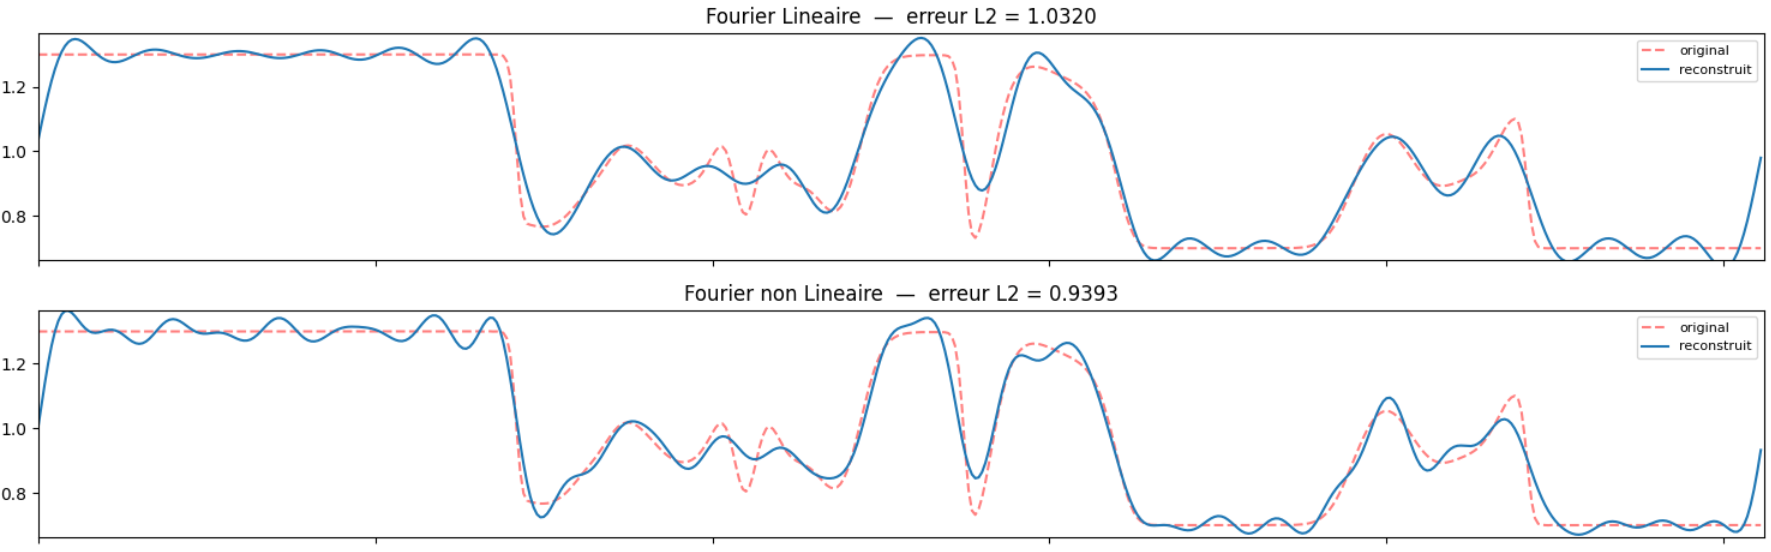
\includegraphics[width=\linewidth]{figures/ch2/fourier.png}
    \end{minipage}

    \caption{Illustration of a Fourier decomposition with 45 modes of a one-dimensional density field.}
    \label{fig:fourier_decomposition}
\end{figure}


In turbulence studies, Fourier analysis is particularly useful because it naturally describes the distribution of energy across spatial scales. Low-frequency modes correspond to large coherent structures, while high-frequency modes represent fine turbulent fluctuations.

\subsection{Advantages for Turbulence Analysis}

Spectral methods possess several important advantages for the analysis of fluid flows. First, Fourier transforms provide compact representations for smooth periodic signals. Second, many physical quantities of interest, such as energy spectra, can be directly expressed in spectral space.

In the context of DNS, pseudo-spectral solvers themselves are often formulated using Fourier representations because of their high numerical accuracy and low dissipation properties. Consequently, Fourier analysis naturally appears as a first candidate for dimensionality reduction and feature extraction.

Furthermore, spectral filtering techniques make it possible to separate structures according to their characteristic scales, which is particularly relevant for turbulent flows exhibiting cascade mechanisms.

\subsection{Limitations for Localized Structures}

Despite their numerous advantages, Fourier representations also exhibit important limitations when dealing with localized or non-smooth structures. Since Fourier basis functions extend over the entire spatial domain, local modifications of the signal affect all spectral coefficients simultaneously. As a consequence, sharp gradients and localized discontinuities generally require a large number of Fourier modes to be accurately reconstructed.

This limitation is closely related to the Gibbs phenomenon, which appears when truncated Fourier series are used to approximate signals containing discontinuities or strong localized variations. Near sharp interfaces, oscillatory artifacts emerge and persist even when increasing the number of retained modes.

\begin{figure}[htbp]
\centering

\includegraphics[width=0.65\textwidth]{figures/ch2/gibbs.png}
\caption{Illustration of the Gibbs phenomenon near a discontinuity reconstructed using a truncated Fourier representation.}
\label{fig:gibbs}
\end{figure}

Although RTI density fields are not strictly discontinuous, they contain steep density gradients, localized interface deformations, and intermittent turbulent structures that exhibit similar reconstruction difficulties. Capturing such localized features using Fourier modes may therefore require a large number of coefficients, reducing compression efficiency and increasing the complexity of the representation.

In addition, Fourier decompositions provide limited spatial localization information. While they accurately describe the global frequency content of the flow, they do not directly indicate where specific structures are located in physical space. This limitation becomes particularly important for turbulent RTI fields, where coherent structures and mixing regions evolve dynamically and remain strongly localized.

These observations motivate the investigation of multi-resolution approaches capable of simultaneously representing both scale-dependent information and spatial localization properties.


\section{Wavelet Transform}

\subsection{Continuous Wavelet Transform}
Wavelet transforms provide a representation framework capable of simultaneously capturing spatial localization and scale-dependent information. The mathematical foundation of wavelet analysis is the \textit{Multi-resolution Analysis} (MRA), introduced by Mallat~\citep[p.~22]{Mallat2009} and Meyer~\citep[p.~22]{Meyer1992}. An MRA is constructed from a scaling function $\phi$, also called the father wavelet, which spans a hierarchy of nested approximation spaces.

Unlike Fourier transforms, which use globally supported sinusoidal basis functions, wavelet transforms employ functions with compact support that can be created by dilation and translation of a mother wavelet $\psi$. We can then define a wavelet as a function of zero mean:
\begin{align}
    \int_{-\infty}^{\infty} \psi(x) dx = 0
\end{align}
The wavelet family is then defined as:
\begin{align}
    \psi_{u,s}(x) = \frac{1}{\sqrt{s}} \psi\left(\frac{x-u}{s}\right)
\end{align}
where $u \in \mathbb{R}$ is the translation parameter and $s > 0$ is the scale parameter. A few examples of wavelet generating functions are shown in Figure \ref{fig:wavelets}.

\begin{figure}[H]
\centering

\includegraphics[width=0.60\textwidth]{figures/ch2/wave.png}
\caption{Examples of wavelet generating functions: Haar, Daubechies, Symlets, and Coiflets.}
\label{fig:wavelets}
\end{figure}

Then, the wavelet transform of a signal $f$, denoted by $\check{f}$ at scale $s$ and position $u$, is defined as:
\begin{align}
    \check{f}(u,s) = \int_{-\infty}^{\infty} f(x) \psi_{u,s}(x) dx \quad \Leftrightarrow \quad \check{f}(u,s) = \langle f, \psi_{u,s} \rangle
\end{align}




\subsection{From Continuous to Discrete Wavelets}

The Continuous Wavelet Transform provides a redundant representation of a signal by evaluating wavelet coefficients over a continuous range of translations and scales. While this formulation offers a powerful theoretical framework for time-frequency and multi-scale analysis, it is not directly suitable for numerical applications. Indeed, the parameters $u$ and $s$ can take infinitely many values, leading to an infinite number of wavelet coefficients for a finite signal.

To obtain a finite and computationally tractable representation, the continuous parameter space is discretized. A common choice consists in sampling the scale and translation parameters on a dyadic grid:
\begin{align}
s_j = 2^{-j},
\qquad
u_{j,n} = n 2^{-j},
\end{align}
where $(j,n) \in \mathbb{Z}^2$. The corresponding family of wavelets becomes
\begin{align}
\psi_{j,n}(x)
=
2^{j/2}
\psi\!\left(2^j x - n\right).
\end{align}

The continuous wavelet transform is then replaced by a discrete set of coefficients
\begin{align}
d_{j,n}
=
\langle f,\psi_{j,n}\rangle,
\end{align}
which quantify the contribution of the signal around position $n$ and scale $2^{-j}$. Unlike the continuous transform, this representation contains a finite number of coefficients for a discretized signal and can therefore be manipulated efficiently on a computer.

The dyadic discretization is closely related to the concept of Multi-resolution Analysis (MRA). In this framework, a hierarchy of nested approximation spaces
\begin{align}
\cdots \subset V_{-1}
\subset V_0
\subset V_1
\subset \cdots
\end{align}
is constructed from the scaling function $\phi$. Each space $V_j$ contains approximations of the signal at resolution $2^{-j}$. The information gained when increasing the resolution from $V_j$ to $V_{j+1}$ is represented by a detail space $W_j$, yielding the fundamental decomposition
\begin{align}
V_{j+1}
=
V_j \oplus W_j.
\end{align}

This relation states that a finer approximation can be obtained by adding the detail information contained in $W_j$ to the coarser approximation $V_j$. Consequently, a signal can be decomposed into a coarse approximation together with a collection of detail coefficients at different scales. This hierarchical representation forms the basis of the Discrete Wavelet Transform and enables efficient multi-scale analysis, compression, and denoising algorithms.



\subsection{Fast Discrete Wavelet Transform in Two Dimensions}

The discretization introduced in the previous section leads to an efficient algorithm for computing wavelet coefficients known as the Fast Wavelet Transform (FWT). Rather than explicitly evaluating inner products with every wavelet basis function, the transform relies on successive filtering operations derived from the Multi-resolution Analysis framework.

For a one-dimensional signal, two complementary filters are applied at each decomposition level:

\begin{itemize}
    \item a low-pass filter associated with the scaling function $\phi$, producing approximation coefficients,
    \item a high-pass filter associated with the wavelet function $\psi$, producing detail coefficients.
\end{itemize}

After filtering, the outputs are downsampled by a factor of two. Denoting by $a_j[n]$ the approximation coefficients at level $j$, the decomposition can be written as

\begin{align}
a_{j+1}[n]
&=
\sum_k h[k] a_j[2n-k], \\
d_{j+1}[n]
&=
\sum_k g[k] a_j[2n-k],
\end{align}

where $h[k]$ and $g[k]$ represent the low-pass and high-pass filter coefficients, respectively. The approximation coefficients capture the large-scale structure of the signal, while the detail coefficients describe localized variations at the corresponding scale. 

Figure \ref{fig:wavelet_1d_example} illustrates the decomposition of a one-dimensional signal using a discrete wavelet transform with Haar wavelets. The original signal is decomposed into approximation and detail coefficients, revealing the hierarchical structure of the data across multiple scales.


\begin{figure}[H]
\centering
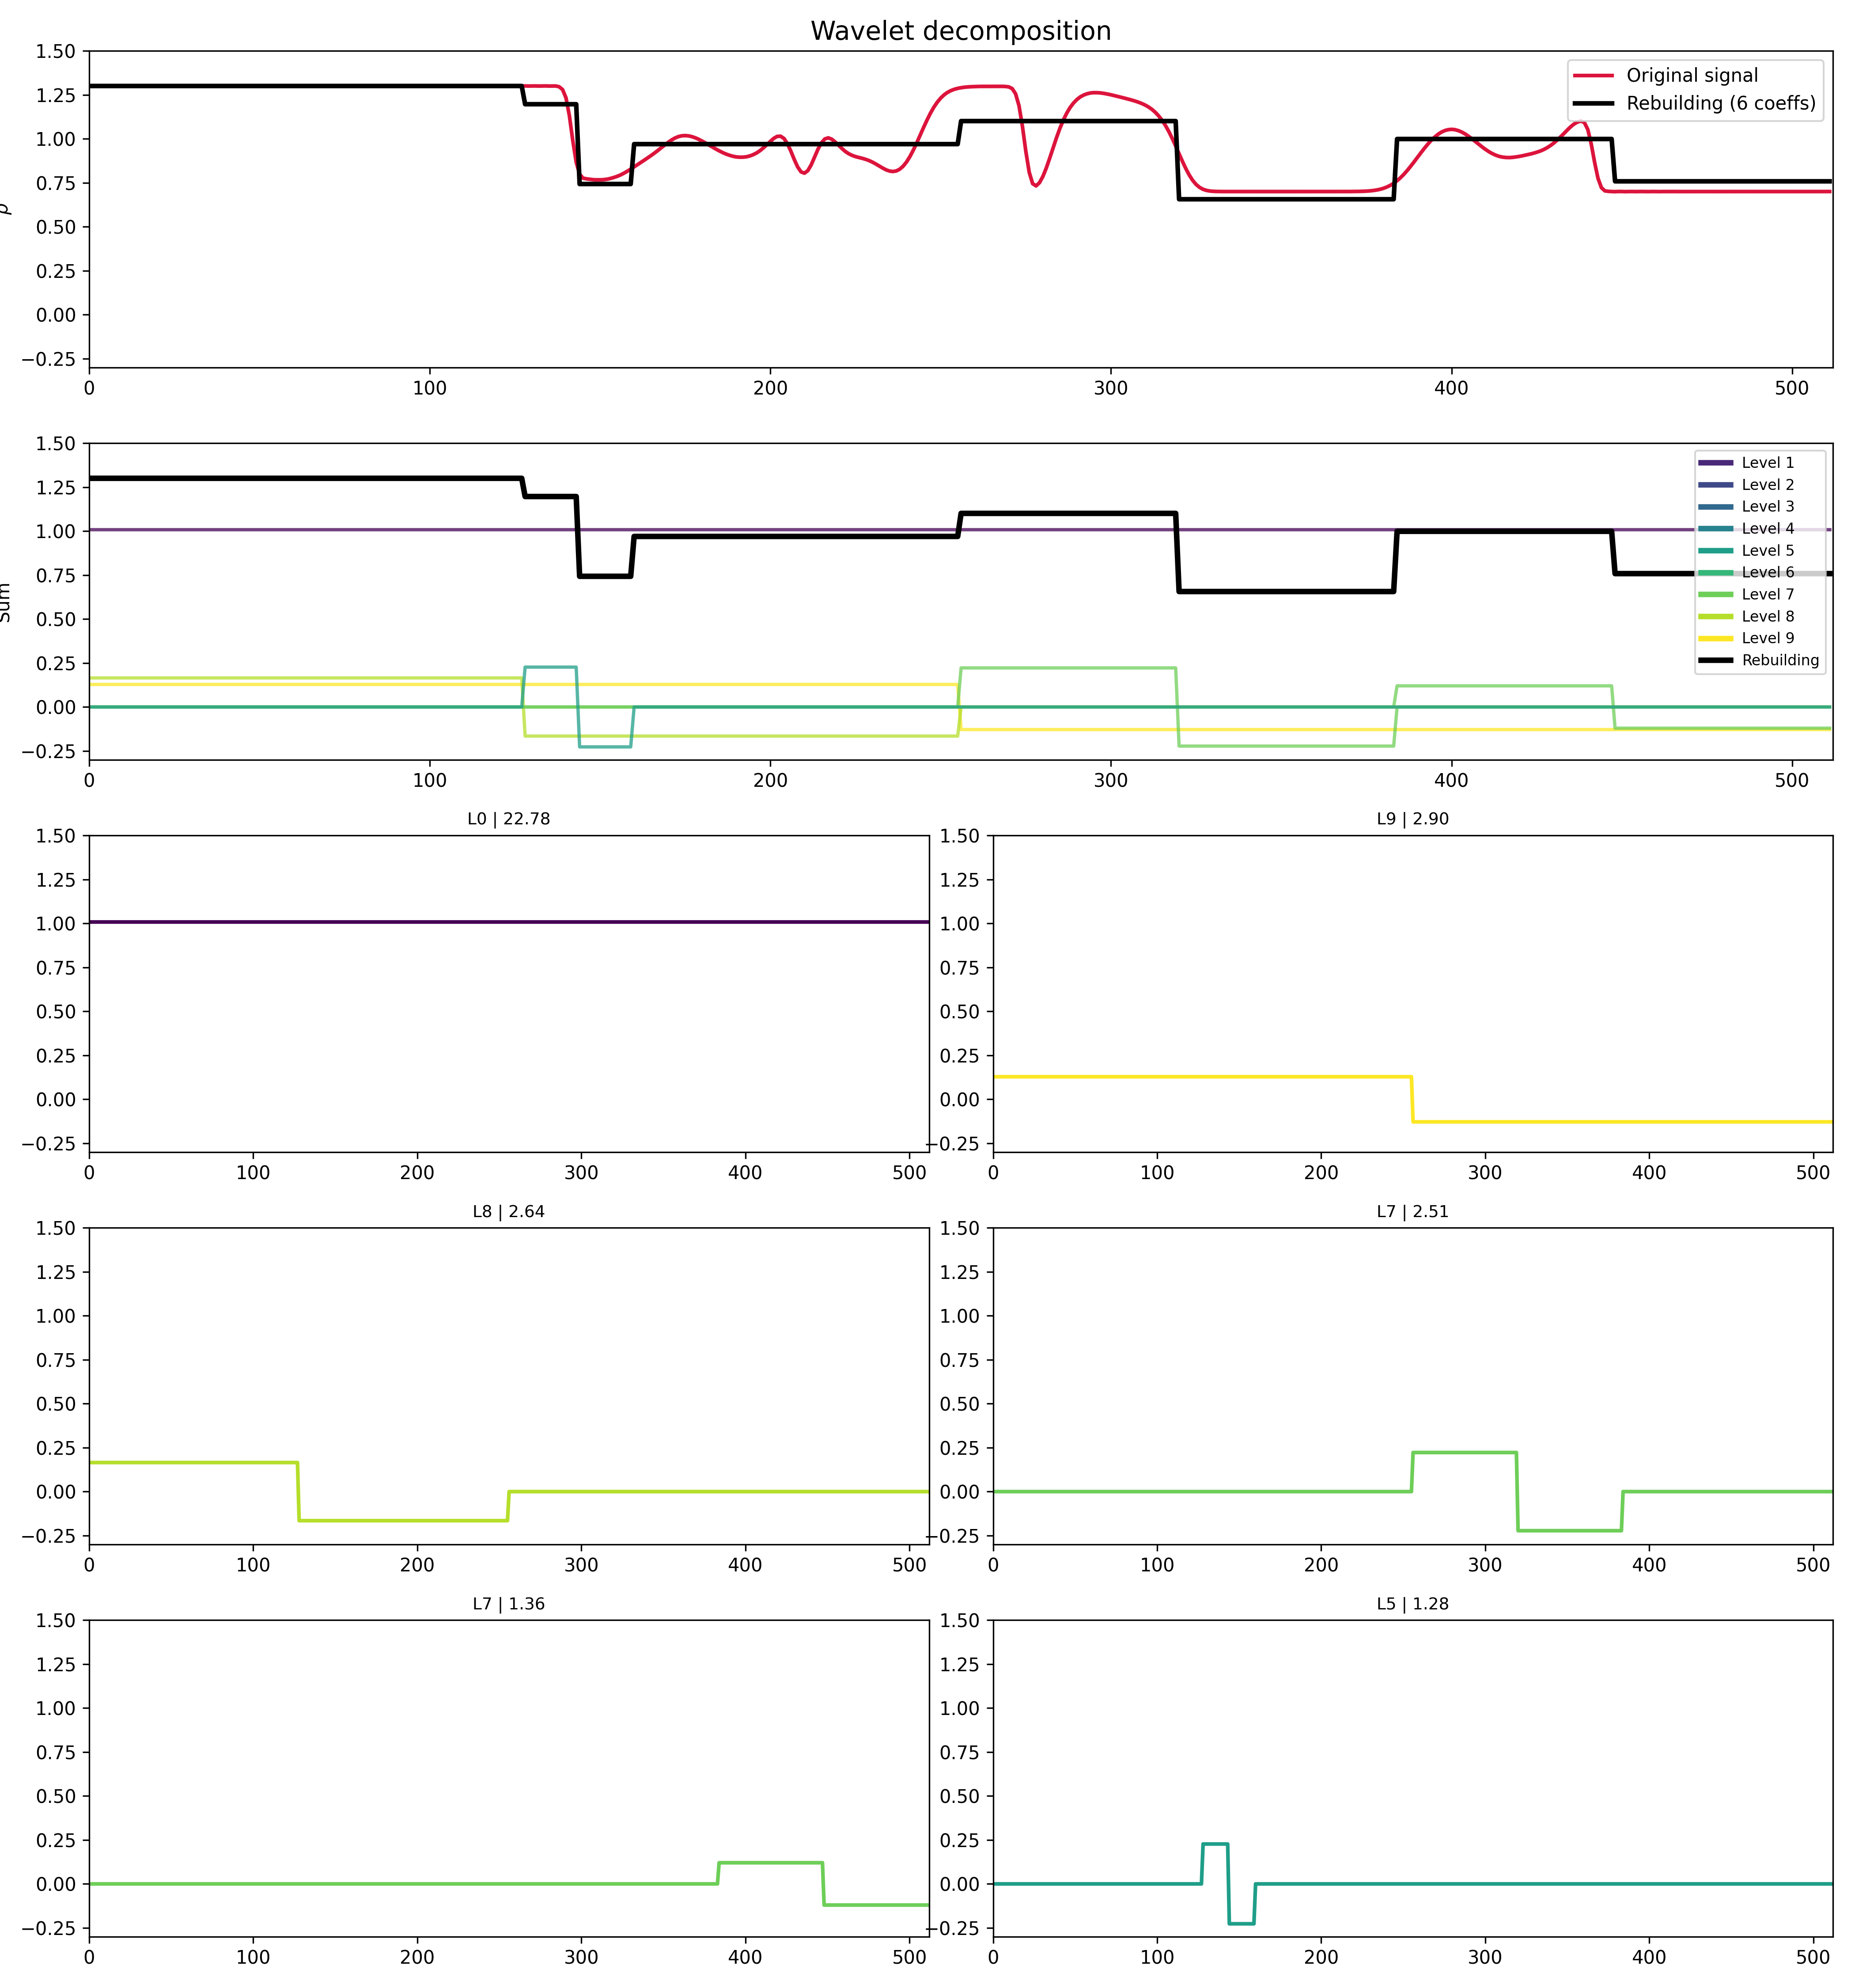
\includegraphics[width=0.85\textwidth]{figures/ch2/1Dwavelets_Decomposition.png}
\caption{Example of a signal decomposition using a one-dimensional discrete wavelet transform, using Haar wavelets.}
\label{fig:wavelet_1d_example}
\end{figure}

For two-dimensional fields, the same principle is applied successively along the horizontal and vertical directions. The image is first filtered row-wise and downsampled, then the resulting intermediate fields are filtered column-wise. This separable construction yields four groups of coefficients:

\begin{align}
LL,\quad LH,\quad HL,\quad HH.
\end{align}

The $LL$ component corresponds to low-pass filtering in both directions and therefore contains a coarse approximation of the original field. The three remaining components contain directional details:

\begin{itemize}
\item $LH$: low-pass horizontally and high-pass vertically,
\item $HL$: high-pass horizontally and low-pass vertically,
\item $HH$: high-pass filtering in both directions.
\end{itemize}

These sub-bands provide a natural separation of structures according to both scale and orientation. Figure \ref{fig:dwt2d_scheme} summarizes the decomposition process, while Figure \ref{fig:dwt2d_example} presents an example applied to a density field from the RTI dataset.

\begin{figure}[H]
\centering

\includegraphics[width=0.8\textwidth]{figures/ch2/wavelet_decomposition.png}
\caption{Schematic representation of a two-dimensional discrete wavelet decomposition.}
\label{fig:dwt2d_scheme}
\end{figure}

\begin{figure}[H]
\centering

\includegraphics[width=0.95\textwidth]{figures/ch2/2DExemple_Masque.png}
\caption{Example of a one-level two-dimensional wavelet decomposition of an RTI density field. The approximation coefficients ($LL$) contain the large-scale structures, while the $LH$, $HL$, and $HH$ sub-bands capture progressively finer directional information.}
\label{fig:dwt2d_example}
\end{figure}

% An important property of this decomposition is that most of the signal energy is generally concentrated within the approximation coefficients, whereas many detail coefficients exhibit relatively small amplitudes. This sparsity property is one of the main reasons why wavelet representations are widely used for compression and multi-scale modeling. In the present work, the $LL$ coefficients are interpreted as a low-resolution representation of the density field and are used as conditioning information for a diffusion model trained to reconstruct the missing detail coefficients. The complete field can then be recovered through the inverse wavelet transform.

\subsection{Compression and Sparsity}

One important property of wavelet representations is their ability to produce sparse decompositions for signals containing localized structures or coherent patterns. A large portion of the signal energy can often be concentrated into a relatively small number of significant coefficients.

This property has been extensively exploited in image compression applications such as JPEG2000, where wavelet decompositions provide efficient representations of natural images while preserving localized features.

In the context of RTI simulations, wavelet sparsity may help reduce the effective dimensionality of the dataset while preserving physically important structures such as interfaces, vortices, and localized mixing regions.

Furthermore, the hierarchical organization of wavelet coefficients appears particularly compatible with the multi-scale nature of turbulence and may therefore provide advantageous representations for generative modeling.

\section{Comparaison and Application to RTI Fields}

\subsection{Comparaison Criteria}
In the context of this work, the main criteria for comparing Fourier and wavelet representations are the number of coefficients required to accurately reconstruct the signal, the ability to capture localized structures and sharp gradients, the effectiveness of separating structures across different scales, and the generalization capabilities to unseen data or different flow regimes. Figure \ref{fig:representation_comparison} illustrates the reconstruction of a two-dimensional Rayleigh--Taylor density field using Fourier, wavelet, and PCA representations with the same number of coefficients. The comparison highlights the differences in capturing sharp gradients and gibbs-like oscillations.
It is also important to note that the PCA is used here as a reference for comparison, but it is not a practical solution for generative modeling since it requires access to the entire training dataset and does not provide extrapolation capabilities for unseen samples.

\begin{figure}[h]
\centering

\includegraphics[width=0.9\textwidth]{figures/ch2/verification_zone_melange.png}
\caption{Comparison of different representations for a two-dimensional Rayleigh--Taylor density field}
\label{fig:representation_comparison}
\end{figure}

For more quantitative comparisons, the reconstruction error is computed as the L2 norm between the original field and its reconstruction. Figure \ref{fig:representation_comparison} shows the evolution of the reconstruction error as a function of the number of coefficients for Fourier, wavelet, and PCA representations. The results indicate that wavelet representations generally provide better reconstruction after a certain number of coefficients having a very steep decrease of the error.

\begin{figure}[h]
\centering
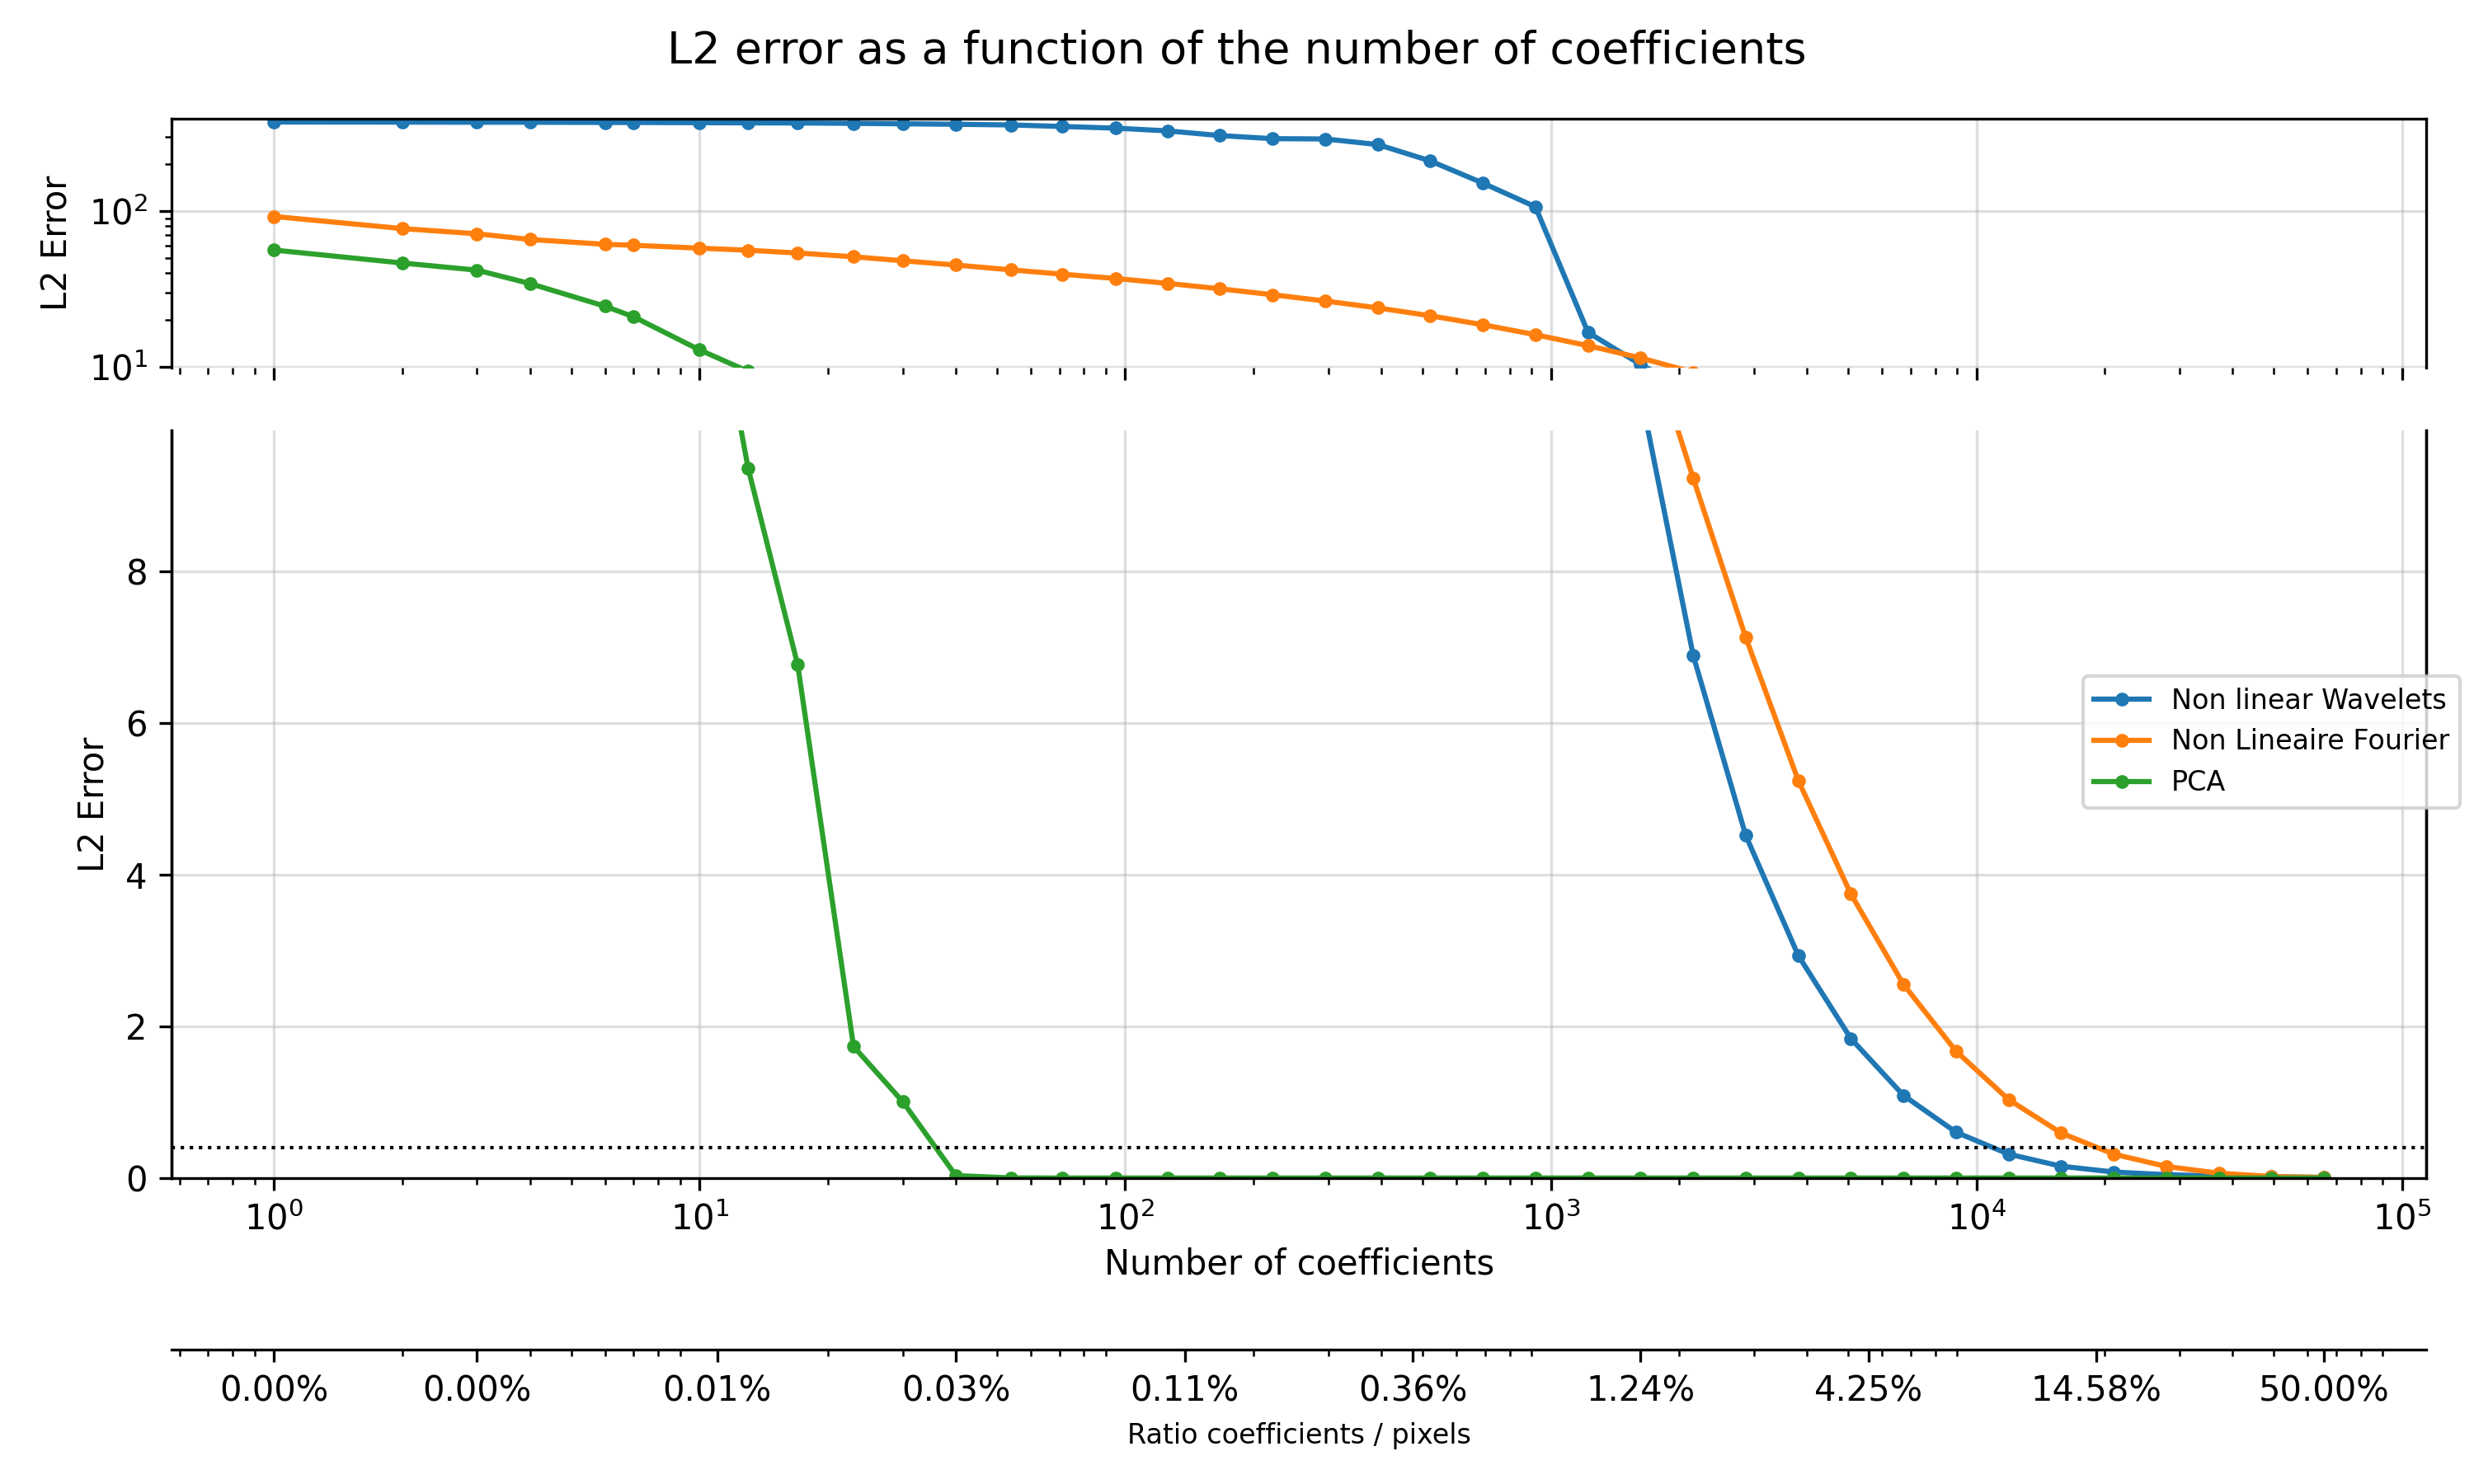
\includegraphics[width=0.65\textwidth]{figures/ch2/dataset2D_Comparaison_des_Erreurs.png}
\caption{Comparison of different representations for a two-dimensional Rayleigh--Taylor density field}
\label{fig:representation_comparison}
\end{figure}

With the same number of coefficients, wavelet representations generally provide better reconstruction of localized structures and sharp gradients compared to Fourier representations. It is for sure less performing than PCA, but it is more robust and independent of the training dataset. The multi-scale nature of wavelet decompositions also allows for a more natural separation of structures across different scales, which is particularly relevant for turbulent RTI flows.